% !TEX encoding = UTF-8 Unicode

% Geoscientific Model Development (gmd)
\documentclass[gmd, manuscript]{copernicus}

% packages
\usepackage{tabu}
\usepackage{booktabs}
\usepackage{graphicx}
\usepackage[export]{adjustbox}
\usepackage[utf8]{inputenc}
\usepackage{listings}
\usepackage[percent]{overpic}

\begin{document}

\title{\lowercase{r.sim.terrain 1.0}: a dynamic landscape evolution model} 

\Author[1]{Brendan Alexander}{Harmon}
\Author[2,3]{Helena}{Mitasova}
\Author[2,3]{Anna}{Petrasova}
\Author[2,3]{Vaclav}{Petras}

\affil[1]{Robert Reich School of Landscape Architecture, Louisiana State University, Baton Rouge, Louisiana, USA}
\affil[2]{Center for Geospatial Analytics, North Carolina State University, Raleigh, North Carolina, USA}
\affil[3]{Department of Marine, Earth, and Atmospheric Sciences, North Carolina State University, Raleigh, North Carolina, USA}

\runningtitle{\lowercase{r.sim.terrain 1.0}: a dynamic landscape evolution model}

\runningauthor{Brendan Harmon}

\correspondence{Brendan Harmon (baharmon@lsu.edu)}

\received{}
\pubdiscuss{}
\revised{}
\accepted{}
\published{}

\firstpage{1}

\maketitle

\begin{abstract}
While there are numerical landscape evolution models
that simulate how steady state flows of water and sediment
reshape topography over long periods of time, 
r.sim.terrain is the first to 
simulate short-term topographic change 
for both steady state and dynamic flow regimes
across a range of spatial scales.
This free and open source, 
GIS-based topographic evolution model
uses empirical models for soil erosion
at watershed to regional scales 
and a physics-based model
for shallow overland water flow and soil erosion 
at subwatershed scales
to compute short-term topographic change. 
This either steady state or dynamic model simulates
how overland sediment mass flows reshape topography
for a range of hydrologic soil erosion regimes
based on topographic, land cover, soil, and rainfall parameters. 
As demonstrated by a case study 
for Patterson Branch subwatershed
on the Fort Bragg military installation in North Carolina,
r.sim.terrain can realistically simulate the development of 
fine-scale morphological features including 
ephemeral gullies, rills, and hillslopes.
Applications include land management, erosion control,
landscape planning, and landscape restoration. 
\end{abstract}

\copyrightstatement{...}

% --------- INTRO FIGURE ---------

\begin{figure}%[H]
\center
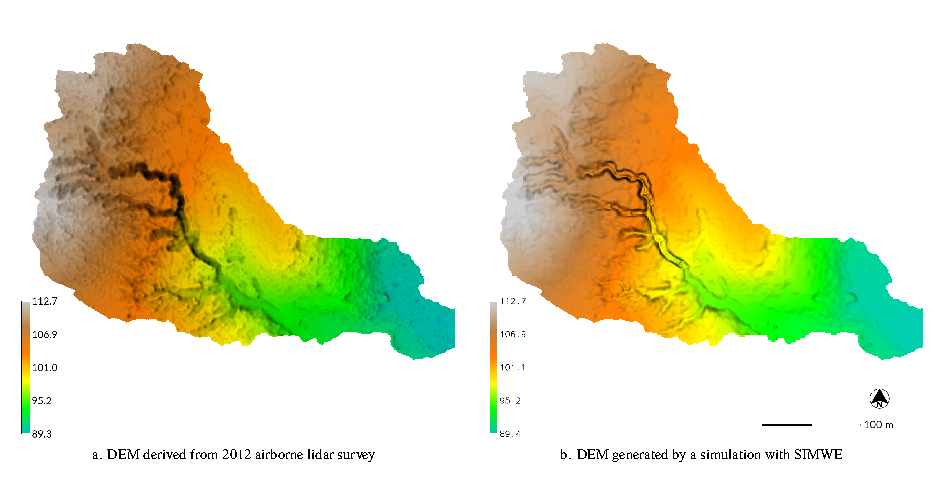
\includegraphics[width=\textwidth,height=0.925\textheight,keepaspectratio]{figures/evolution.pdf}
\caption{
The digital elevation model (DEM) 
before (a.) and after (b.)
simulated landscape evolution with
r.sim.terrain. 
This simulation used the SIMWE model
for a 120~\unit{min} rainfall event with 25~\unit{mm~hr}$^{-1}$
in a transport limited soil erosion regime at steady state.
In the evolved DEM (b.)
the gully channel has widened 
with depositional ridges forming along its thalweg.}
\label{fig:evolution}
\end{figure}

% --------- BODY ---------

\introduction
Landscape evolution models represent how the surface of the earth changes 
over time in response to physical processes. 
Most studies of landscape evolution have been descriptive, 
but a number of numerical landscape evolution models 
have been developed that simulate elevational change over time 
\citep{Temme2013}. 
% numerical models
Numerical landscape evolution models
such as the Channel-Hillslope Integrated Landscape Development (CHILD) model 
\citep{Tucker2001} 
and SIBERIA \citep{Willgoose2005}
simulate steady state flows over long temporal scales. 
% recent development
\href{http://landlab.github.io/}{Landlab},
a new Python library for numerically modeling Earth surface processes
\citep{Hobley2017},
has components for simulating landscape evolution such as the 
Stream Power with Alluvium Conservation and Entrainment (SPACE) 
model \citep{Shobe2017}.
% gis-based models
While Geographic Information Systems (GIS)
support efficient data management, 
spatial and statistical modeling and analysis, 
and visualization,
there are few GIS-based soil erosion models or landscape evolution models
(see Tables~\ref{table:erosion_models}-\ref{table:evolution_models}).
% research questions
Furthermore there are still major research questions 
to address in the theoretical foundations of erosion modeling 
such as how erosional processes scale over time and space 
and how sediment detachment and transport interact \citep{Mitasova2013}. 
% dynamic evolution
While most numerical landscape evolution models 
simulate peak flows at steady state
(see Table~\ref{table:evolution_models}),
short-term erosional processes like gully formation can be dynamic
with significant morphological changes happening within minutes
before flows reach steady state. 
A dynamic landscape evolution model is needed to study
fine-scale spatial and short-term temporal erosional processes
such as gully formation and the development of microtopography. 


% steady state versus dynamic
At the beginning of a rainfall event 
the overland water flow regime is dynamic -- 
its depth changes at a variable rate over time and space. 
If the intensity of rainfall continues to change throughout the event
then the flow regime will remain dynamic. 
% steady state
If, however, the overland flow reaches a peak rate
then the hydrologic regime is considered to be at steady state.
At steady state:
% steady state eq.
\begin{equation}
\label{eq:steady_state}
{\partial h(x,y,t) \over \partial t} = 0
\end{equation}
%
{\small
\noindent
where: \\
\noindent
\hspace*{0.5em} $(x,y)$ is the position [\unit{m}]\\
\hspace*{0.5em} $t$ is the time [\unit{s}]\\
\hspace*{0.5em} $h(x,y,t)$ is the depth of overland flow [\unit{m}]\\
}

% gully formation
Gullies are eroded, steep banked channels 
formed by ephemeral, concentrated flows of water.
A gully forms when overland waterflow
converges in a knickzone
-- a concave space with steeper slopes than its surroundings 
\citep{Zahra2017} -- 
during intense rainfall events.  
When the force of the water flow concentrated in the knickzone
is enough to detach and transport large amounts of sediment,
an incision begins to form at the apex of the knickzone 
-- the knickpoint or headwall.
As erosion continues the knickpoint begins to migrate upslope
and the nascent gully channel widens,
forming steep channel banks. 
Multiple incisions initiated by different knickpoints 
may merge into a gully channel
and multiple channels may merge 
into a branching gully system \citep{Mitasova2013}. 
This erosive process is dynamic; 
the morphological changes drive further changes 
in a positive feedback loop
until water flow reaches steady state. 
When the gully initially forms 
the soil erosion regime should be detachment capacity limited
with the concentrated flow of water in the channel of the gully 
detaching large amounts of sediment 
and transporting it to the foot of the gully, 
potentially forming a depositional fan. 
After the initial formation of the gully
the soil erosion regime may switch
to erosion-deposition if the intensity of rainfall decreases.
Subsequent rainfall events may trigger further 
knickpoint formation and upslope migration, 
channel incision and widening, and
depositional fan and ridge formation. 
Between high intensity rainfall events, 
lower intensity events and gravitational diffusion
may gradually smooth the shape of the gully. 
Eventually, if detachment capacity 
significantly exceeds transport capacity, 
the gully may fill with sediment. 

% gully monitoring
Gully erosion rates and evolution
can be monitored in the field 
or modeled on the computer. 
% field methods
Field methods include
dendrogeomorphology \citep{Malik2008} and 
permanent monitoring stakes for recording erosion rates, 
extensometers for recording mass wasting events, 
weirs for recording water and suspended sediment discharge rates, 
and time series of surveys using 
total station theodolites \citep{Thomas2004},
unmanned aerial systems (UAS),
airborne lidar, and terrestrial lidar \citep{Starek2011,Bechet2016}.
% high resolution topographic data
With terrestrial lidar, airborne lidar and 
UAS photogrammetry
there is now sufficient resolution topographic data 
to morphometrically analyze and 
numerically model fine-scale landscape evolution in GIS
including processes such as gully formation 
and the development of microtopography. 
% gully simulation
Gully erosion has been simulated with 
the Revised Universal Soil Loss Equation Version 2 (RUSLER)
in conjunction with the Ephemeral Gully Erosion Estimator (EphGEE)
\citep{Dabney2014},
while gully evolution
has been simulated for detachment capacity limited erosion regimes
with the Simulation of Water Erosion (SIMWE) model
\citep{Koco2011, Mitasova2013}. 
Now numerical landscape evolution models 
that can simulate 
steady state and dynamic flow regimes
and can dynamically switch between soil erosion regimes 
are needed to study 
fine-scale spatial and short-term temporal erosional processes.

% aim
The numerical landscape evolution model 
r.sim.terrain was developed to 
simulate the spatiotemporal evolution of landforms
caused by shallow overland water and sediment flows
at spatial scales ranging from
square meters to kilometers
and temporal scales ranging from minutes to years. 
% objectives
This open source, GIS-based landscape evolution model can
simulate either steady state or dynamic flow regimes, 
dynamically switch between soil erosion regimes, and
simulate the evolution of fine-scale morphological features 
such as ephemeral gullies
(Figure~\ref{fig:evolution}).
% questions
It was designed as a research tool for
studying how erosional processes scale over time and space,
comparing empirical and process-based models, 
comparing steady state and dynamic flow regimes, and
studying the role of dynamic flow regimes 
in fine-scale morphological change. 
% testing
r.sim.terrain was tested with 
a subwatershed scale (450~\unit{m}$^{2}$) case study
and the simulations were compared against 
a time-series of airborne lidar surveys.

\section{r.sim.terrain}
The process-based, spatially distributed 
landscape evolution model r.sim.terrain
simulates topographic changes
caused by shallow, overland water flow
across a range of spatiotemporal scales and soil erosion regimes
using either
the Simulated Water Erosion (SIMWE) model, 
the 3-Dimensional Revised Universal Soil Loss Equation (RUSLE 3D) model,
or the Unit Stream Power Erosion Deposition (USPED) model.  
% simwe
SIMWE is a physics-based simulation
that uses a Monte Carlo path sampling method
to solve the water and sediment flow equations 
for detachment limited, transport limited, and variable erosion-deposition 
soil erosion regimes \citep{Mitasova2004}. 
With SIMWE 
r.sim.terrain
uses the modeled flow of sediment 
-- a function of water flow and soil detachment and transport parameters -- 
to estimate net erosion and deposition rates. 
% rusle3d
RUSLE3D is an empirical equation for sediment flows 
in detachment capacity limited soil erosion regimes \citep{Mitasova1996}. 
With RUSLE3D
r.sim.terrain
uses an event-based erosivity factor, 
the slope, the flow accumulation, and a 3D topographic factor
to model sediment flow. 
% usped
USPED is an empirical equation for net erosion and deposition 
in transport capacity limited soil erosion regimes. 
With USPED 
r.sim.terrain
uses an event-based erosivity factor, 
the slope and aspect, the flow accumulation, and a 3D topographic factor
to model erosion-deposition as the
the divergence of sediment flows. 
% evolution
For each of the models 
topographic change is derived at each time step
from the sediment flow or net erosion-deposition rate
and gravitational diffusion.
% regimes
The r.sim.terrain model
can simulate either steady state or dynamic flow regimes.
During simulations with SIMWE 
r.sim.terrain
can switch between 
detachment limited, transport limited, and variable erosion-deposition 
soil erosion regimes.

% capabilities
The r.sim.terrain model
can simulate the evolution of gullies
including processes such as 
knickpoint migration,
channel incision, 
channel widening, 
aggradation, and
scour pool and 
depositional ridge formation
along the thalweg of the gully. 
% applications
Applications include 
geomorphological research,
erosion control, 
landscape restoration, 
and scenario development 
for landscape planning and management.
% scale
This model can simulate landscape evolution 
over a wide range of spatial scales 
from small watersheds 
less than ten square kilometers
with SIMWE
to regional watersheds
of hundreds of square kilometers
with USPED or RULSE3D,
although it does not model fluvial processes. 
% implementation
This model has been implemented 
as a Python add-on module 
for the free, open source
\href{https://grass.osgeo.org/}{Geographic Resources Analysis Support System (GRASS) GIS}
\citep{GRASS}. 
The source code is available at 
\url{https://github.com/baharmon/landscape\_evolution} 
under the GNU General Public License v2.
% parallel processing
It supports multithreading and parallel processing
to efficiently compute simulations 
using large, high resolution topographic datasets.
%
The landscape evolution model 
can be installed in GRASS GIS as an add-on module 
with the command: 
\begin{verbatim}
g.extension r.sim.terrain
\end{verbatim}

% -------------------------- TABLE OF MODELS -----------------------------

% table of erosion models
\begin{table*}
\small
\caption{Geospatial soil erosion models}
\begin{tabu} to \textwidth {XXXXXl}
\toprule
Model & Spatial scale &  Temporal scale & Representation & Implementation & Reference\\
\midrule
RUSLE3D & regional & continuous & raster & map algebra & \citep{Mitasova1996}\\
USPED & watershed & continuous & raster & map algebra & \citep{Mitasova1996}\\
\href{https://grass.osgeo.org/grass74/manuals/r.sim.sediment.html}{SIMWE} & watershed & event -- & raster & \href{https://grass.osgeo.org/grass74/manuals/r.sim.sediment.html}{GRASS modules} & \citep{Mitas1998}\\
&& continuous\\
\href{http://geowepp.geog.buffalo.edu/}{GeoWEPP} & watershed & continuous & raster & \href{http://geowepp.geog.buffalo.edu/}{ArcGIS module} & \citep{Flanagan2013}\\
\href{https://www.tucson.ars.ag.gov/agwa/}{AGWA}  & watershed & event -- & vector & \href{https://www.tucson.ars.ag.gov/agwa/}{ArcGIS module} & \citep{Guertin2015}\\
&& continuous\\
\bottomrule
\\
\end{tabu}
\label{table:erosion_models}
\end{table*}

% table of landscape evolution models
\begin{table*}
\small
\caption{Topographic evolution models}
\begin{tabu} to \textwidth {XXXXXll}
\toprule
Model & Spatial scale &  Temporal scale & Representation & Dynamics & Implementation & Reference\\
\midrule
\href{https://csdms.colorado.edu/wiki/Model:CHILD}{CHILD} & regional & continuous & mesh & steady state & \href{https://csdms.colorado.edu/wiki/Model:CHILD}{C++ program} & \citep{Tucker2001}\\
\href{https://csdms.colorado.edu/wiki/Model:SIBERIA}{SIBERIA} & regional & continuous & raster & steady state & \href{https://csdms.colorado.edu/wiki/Model:SIBERIA}{Fortran prog.} & \citep{Willgoose2005}\\
\href{https://grass.osgeo.org/grass74/manuals/addons/r.landscape.evol.html}{r.landscape.evol}  & regional & continuous & raster &  steady state & \href{https://grass.osgeo.org/grass74/manuals/addons/r.landscape.evol.html}{GRASS module} & \citep{Barton2010}\\
\href{https://github.com/landlab/}{Landlab} & regional & continuous & raster + mesh & steady state & \href{https://github.com/landlab/}{Python library} & \citep{Hobley2017}\\
\href{https://github.com/baharmon/landscape_evolution}{r.sim.terrain} & watershed -- & event -- & raster & dynamic -- & \href{https://github.com/baharmon/landscape_evolution}{GRASS module} &\\
& regional & continuous && steady state & &\\
\bottomrule
\\
\end{tabu}
\label{table:evolution_models} 
\end{table*}

% -------------------------- MODEL FIGURE -----------------------------

% model figure
\begin{figure}
\center
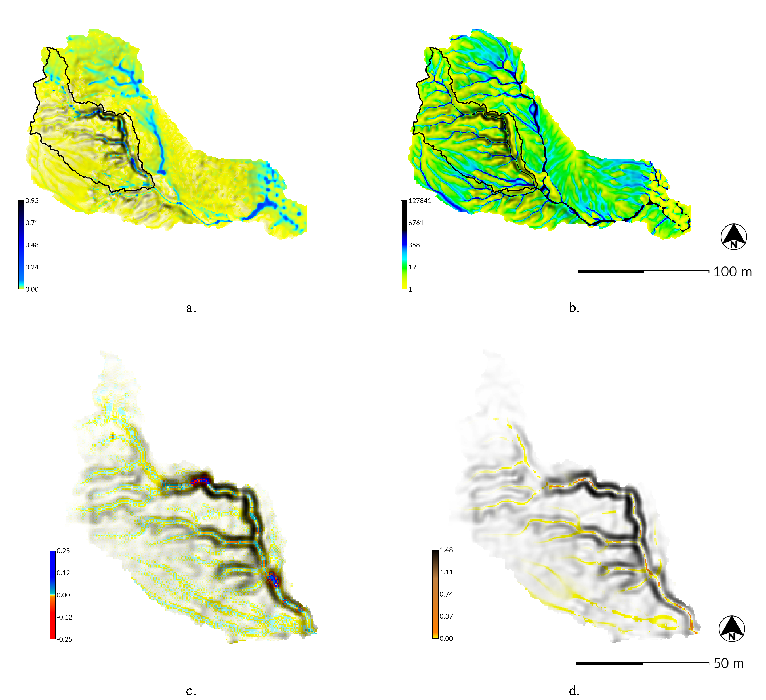
\includegraphics[width=\textwidth,height=0.95\textheight,keepaspectratio]{figures/models.pdf}
\caption{Water and sediment flows simulated by SIMWE 
for a 10~\unit{min} event with 50~\unit{mm~hr}$^{-1}$
and by RUSLE3D with a R-factor of 310
}
\label{fig:models}
\end{figure}

% -------------------------- EROSION-DEPOSITION -----------------------------
\subsection{Simulation of water erosion model} \label{simwe}
% simwe intro
SIMWE -- the Simulation of Water Erosion model -- 
is a physics-based simulation of shallow overland water and sediment flow
that uses a path sampling method to solve the continuity and momentum equations 
with a 2D diffusive wave approximation 
\citep{Mitas1998,Mitasova2004}.
SIMWE has been implemented in GRASS GIS as the modules 
r.sim.water
and r.sim.sediment.

% overview
In SIMWE mode 
for each time step
r.sim.terrain
determines the soil erosion regime,
simulates water and sediment flows, 
and then evolves the topography. 
% erdep
In an variable erosion-deposition regime 
the model 
computes the partial derivatives of the topography,
simulates shallow water flow and erosion-deposition,
and then evolves the topography based on the erosion-deposition rate
and gravitational diffusion.
% transport limited
The same process is used in
a transport capacity limited regime,
except that the topography is evolved based on 
the transport limited erosion-deposition rate
and gravitational diffusion.
% detachment  limited
In a detachment capacity limited regime
the model instead
computes the partial derivatives of the topography,
simulates shallow water flow and sediment flow,
and then evolves the topography based on the sediment flow rate
and gravitational diffusion.
% dynamic versus steady state
The model simulates dynamic landscape evolution 
when the time step is less than the travel time 
for a drop of water or a particle of sediment to cross the landscape.
With longer time steps the model simulates steady state dynamics. 

% ------------------------------------------------------------------------------

\subsubsection{Erosion regime}

% Erosion regime
This model can switch erosion regimes at each time step
based on the rainfall intensity ($i_r$)
and the balance of the sediment detachment capacity ($D_c$)
and the sediment transport capacity ($T_c$)
represented by the first order reaction term $\sigma$, 
which depends on soil and landcover properties.
The detachment capacity is the maximum potential 
detachment rate by overland flow, while
the sediment transport capacity 
is the maximum potential sediment flow rate.
When rainfall intensity is very high ($i_r \geq 60 \unit{mm~hr}^{-1}$)
or $\sigma$ is low ($\sigma \leq 0.01 \unit{m}^{-1}$),
then the regime is detachment capacity limited. 
%
When rainfall intensity is not very high ($i_r < 60 \unit{mm~hr}^{-1} $)
and $\sigma$ is high ($\sigma \geq 100 \unit{m}^{-1}$),
then the regime is transport capacity limited. 
%
When rainfall intensity is not very high 
($i_r<60 \unit{mm~hr}^{-1}$)
and $\sigma$ is neither high nor low 
($ 0.01 \unit{m}^{-1}< \sigma < 100 \unit{m}^{-1}$),
then there is an variable erosion-deposition regime. \\
% erosion regime eq.
\begin{equation}
\label{eq:regime}
\sigma = {D_c \over T_c}
\end{equation}
{\small
\noindent
where: \\
\noindent
\hspace*{0.5em} $\sigma$  is a first order reaction term [$\unit{m}^{-1}$]\\
\hspace*{0.5em} $D_c$ is the sediment detachment capacity [$\unit{kg~m}^{-1}s^{-1}$]\\
\hspace*{0.5em} $T_c$ is the sediment transport capacity [$\unit{kg~m}^{-1}s^{-1}$]\\
}

% ------------------------------------------------------------------------------

\subsubsection{Shallow water flow}

% Shallow water flow
The SIMWE model
simulates shallow overland water flow
controlled by spatially variable topographic, soil, landcover, 
and rainfall parameters
by solving the continuity and momentum equations 
for steady state water flow with a path sampling method
(Fig.~\ref{fig:models}a). 
Shallow water flow $q$ can be approximated by
the bivariate form of the St.~Venant equation:
% shallow water flow eq.
\begin{equation}
\label{eq:water}
{\partial h \over \partial t} =
 i_e - \nabla ~ q
\end{equation}
{\small
\noindent
where: \\
\noindent
\hspace*{0.5em} $x, y$ is the position [\unit{m}]\\
\hspace*{0.5em} $t$ is the time [\unit{s}] \\
\hspace*{0.5em} $h$ is the depth of overland flow [\unit{m}]\\
\hspace*{0.5em} $i_e$ is the rainfall excess [\unit{m~s^{-1}}] \\
\hspace*{0.5em} (i.e.~rainfall intensity $-$ infiltration $-$ vegetation intercept)\\
\hspace*{0.5em} $\nabla$ is the divergence of the flow vector field\\
\hspace*{0.5em} $q$ is the water flow per unit width [$\unit{m}^2~\unit{s}^{-1}$]. \\
}

\noindent
Diffusive wave effects can be approximated
so that water can flow through depressions 
by integrating a diffusion term 
$ \propto \nabla^2 [h^{5/3}]$
into the solution of the continuity and momentum equations 
for steady state water flow.
This equation is solved using a 
Green's function Monte Carlo path sampling method. 
%  diffuse wave eq.
\begin{equation}
\label{eq:difwater}
-{\varepsilon\over 2 }\nabla^2 [h^{5/3}]
+\nabla ~ [ h~v] = i_e
\end{equation}
{\small
\noindent
 where: \\
 \noindent
 \hspace*{0.5em} $\varepsilon$ is a spatially variable diffusion coefficient. \\
}

% ------------------------------------------------------------------------------

\subsubsection{Sediment flow}

% Sediment flow
In SIMWE the sediment flow rate $q_s$ is estimated
as a function of water flow and sediment concentration
\citep{Mitas1998}
(Fig.~\ref{fig:models}b): 
%sediment flow equation
\begin{equation}\label{eq:sedflow} 
q_s = \rho_s ~ q
\end{equation}
{\small
\noindent
where: \\
\hspace*{0.5em} $q_s$ is the sediment flow rate per unit width [\unit{kg~m}$^{-1}$~\unit{s}$^{-1}$]\\
\hspace*{0.5em} $\rho_s$ is sediment mass density [\unit{kg~m}$^{-3}$].\\
}

% ------------------------------------------------------------------------------

\subsubsection{Erosion-deposition}

% Erosion-deposition
In SIMWE 
the net erosion-deposition rate is estimated
using the bivariate form of sediment continuity equation
to model sediment storage and flow 
based on effective sources and sinks
(Fig.~\ref{fig:models}c). 
Net erosion-deposition $d_s$
-- the difference between sources and sinks --
is approximated by
the steady state sediment flow equation with diffusion:
% erosion-deposition equation
\begin{equation}\label{eq:sediment} 
d_s = 
{\partial [\rho_s ~ h] \over \partial t} +
\nabla~q_s
\end{equation}
{\small
\noindent
where: \\
\hspace*{0.5em} $d_s$ is net erosion-deposition [\unit{kg~m}$^{-2}$~\unit{s}$^{-1}$].\\
}

% ------------------------------------------------------------------------------

\subsubsection{Landscape evolution}

% Landscape evolution
The simulated change in elevation $\Delta z$
due to water erosion and deposition
is a function of
the change in time, the net erosion-deposition rate, and the sediment mass density 
\citep{Mitasova2013}:
% landscape evolution equation
\begin{equation}
\label{eq:evolution} 
{\Delta z = \Delta t ~ d_s ~ \rho_s^{-1} }
\end{equation}

% detachment limited landscape evolution
\noindent
In a detachment limited erosion regime
the simulated change in elevation $\Delta z$
is a function of
the change in time, the sediment flow rate, and the mass of water carried sediment per unit area
\citep{Mitasova2013}:
% change in elevation (m) = change in time (s) * sediment flux (kg/ms) / mass of sediment per unit area (kg/m^2)
\begin{equation}
\label{eq:flux_evolution} 
{\Delta z = \Delta t ~ q_s~ \varrho_s^{-1} } 
\end{equation}
{\small
\noindent
where: \\
\noindent
\hspace*{0.5em} $\varrho_s$ is the mass of sediment per unit area [\unit{kg ~ m}$^{-2}$].\\
}


% ------------------------------------------------------------------------------

% gravitational diffusion
\noindent
Gravitational diffusion is then applied to the evolved topography
to simulate the settling of sediment particles. 
The simulated change in elevation $\Delta z$ %$\Delta z(x,y,t)$
due to gravitational diffusion 
is a function of the change in time, the sediment mass density, 
the gravitational diffusion coefficient, and topographic divergence 
-- i.e.~the sum of the second order derivatives of elevation
\citep{thaxton2004}:
% change in elevation (m) = elevation (m) - (change in time (s) / sediment mass density (kg/m^3) * gravitational diffusion coefficient (m^2/s) * divergence (m^-1))
\begin{equation}
\label{eq:grav_diffusion} 
{\Delta z = \Delta t ~ \rho_s^{-1} ~ \varepsilon_g ~ \nabla}
\end{equation}
{\small
\noindent
where: \\
\noindent
\hspace*{0.5em} $\varepsilon_g$ is the gravitational diffusion coefficient [\unit{m}$^{2}$~\unit{s}$^{-1}$]\\ \hspace*{0.5em} $\nabla$ is the topographic divergence [\unit{m}$^{-1}$].\\
}

% -------------------------------- RUSLE --------------------------------
\subsection{Revised universal soil loss equation 3D model}
\label{rusle_model}
The Revised Universal Soil Loss Equation for Complex Terrain (RUSLE3D) 
is an empirical equation for computing erosion 
in a detachment capacity limited soil erosion regime
for watersheds with complex topography \citep{Mitasova1996}. 
It is based on 
the Universal Soil Loss Equation (USLE),
an empirical equation for estimating the average
sheet and rill soil erosion from rainfall and runoff
on agricultural fields and rangelands with simple topography 
\citep{Wischmeier1978}. 
It models erosion dominated regimes without deposition
in which sediment transport capacity is 
uniformly greater than detachment capacity.
As an empirical equation the predicted soil loss 
is spatially and temporally averaged. 
In USLE soil loss per unit area is determined by 
an erosivity factor $R$,
a soil erodibility factor $K$, 
a slope length factor $L$,
a slope steepness factor $S$,
a cover management factor $C$,
and a prevention measures factor $P$.
These factors are empirical constants derived 
from an extensive collection of measurements 
on 22.13 \unit{m} standard plots with an average slope of 9$\%$.  
RUSLE3D was designed to account for more complex, 3D topography 
with converging and diverging flows. 
In RUSLE3D the topographic potential for erosion at any given point 
is represented by a 3D topographic factor $LS_{3D}$,
which is a function of the upslope contributing area 
and the angle of the slope. 

In this spatially and temporally distributed model 
RUSLE3D is modified by the use of a 
event-based r-factor derived from the rainfall intensity 
at each time step.
For each time step
this model computes the parameters for RUSLE3D -- 
an event-based erosivity factor,
the slope of the topography, the flow accumulation, and
the 3D topographic factor -- and then
solves the RUSLE3D equation for sediment flow. 
The sediment flow is used to simulate landscape evolution 
in a detachment capacity limited soil erosion regime.

% RESOURCES
% https://ncsu-geoforall-lab.github.io/erosion-modeling-tutorial/erdep_theory.html
% http://www4.ncsu.edu/~hmitaso/gmslab/reports/CerlErosionTutorial/denix/denixstart.html

% ------------------------------------------------------------------------------

\subsubsection{Event-based erosivity factor}

The erosivity factor $R$ 
in USLE and RUSLE 
is the combination of the total energy 
and peak intensity of a rainfall event,
representing the interaction 
between the detachment of sediment particles
and the transport capacity of the flow. 
It can be calculated as the product of the 
the kinetic energy of the rainfall event $E$
and its maximum 30 \unit{min} intensity $I_{30}$
\citep{Brown1987,Renard1997}.
In this model, however, the erosivity factor
is derived at each time step as a function of
kinetic energy, rainfall volume, rainfall intensity, and time.
First rain energy is derived from rainfall intensity \citep{Brown1987}:
%
\begin{equation}
\label{eq:rain_energy}
{e_r = 0.29 ~ (1.-0.72 ~ exp(-0.05 ~ i_r))}
\end{equation}
%
{\small
\noindent
where: \\
\noindent
\hspace*{0.5em} $e_r$is unit rain energy [\unit{MJ~ha}$^{-1}$~\unit{mm}${^-1}$]\\
\hspace*{0.5em} $i_r$ is rainfall intensity [\unit{mm~h}$^{-1}$].\\
}

\noindent
Then the event-based erosivity index $R_e$ 
is calculated as the product of 
unit rain energy, rainfall volume, rainfall intensity, and time: 
\begin{equation}
\label{eq:erosivity_index}
{R_e = e_r ~ v_r ~ i_r ~ t_r}
\end{equation}
%
{\small
\noindent
where: \\
\hspace*{0.5em} $R_e$ is the event-based erosivity index [\unit{MJ~mm~ha}$^{-1}$~\unit{hr}$^{-1}$]\\
\hspace*{0.5em} $v_r$ is the rainfall volume [\unit{mm}] derived from ${v_r = i_r~t_r}$\\
\hspace*{0.5em} $t_r$ is the time interval [\unit{s}].
}

% ------------------------------------------------------------------------------

\subsubsection{Flow accumulation}
%
The upslope contributing area per unit width 
is determined by flow accumulation times grid cell width
(Fig.~\ref{fig:models}d). 
Flow accumulation is calculated using 
a multiple flow direction algorithm \citep{Metz2009} 
based on $A^{T}$ least cost path searches \citep{Ehlschlaeger1989}. 
The multiple flow direction algorithm 
implemented in GRASS GIS as the module r.watershed
is computationally efficient and can
navigate nested depressions and other obstacles. 

% ------------------------------------------------------------------------------

\subsubsection{3D topographic factor}
%
The 3D topographic factor $LS_{3D}(x,y)$
is calculated as a function of 
the flow accumulation,
representing the upslope contributing area,
and the slope 
(Fig.~\ref{fig:models}e). 
%
The empirical coefficients $m$ and $n$
for the upslope contributing area 
and the slope
can range from 0.2 to 0.6
and 1.0 to 1.3 respectively
with low values representing dominant sheet flow
and high values representing dominant rill flow.
%
\begin{equation}
\label{eq:ls_factor}
{LS_{3D} = (m+1.0) ~ (a(x,y) ~ a_0^{-1})^{m} ~ (sin(\beta) ~ \beta_0^{-1})^{n}}
\end{equation}
%
{\small
\noindent
where: \\
\noindent
\hspace*{0.5em} $LS_{3D}$ is the dimensionless topographic (length-slope) factor\\
\hspace*{0.5em} $a$ is upslope contributing area per unit width [\unit{m}]\\
\hspace*{0.5em} $a_0$ is the length of the standard USLE plot [22.1 \unit{m}]\\
\hspace*{0.5em} $\beta$ is the angle of the slope [$\degree$]\\
\hspace*{0.5em} $m$ is an empirical coefficient\\
\hspace*{0.5em} $n$ is an empirical coefficient\\
\hspace*{0.5em} $\beta_0$ is the slope of the standard USLE plot [0.09$\degree$]\\
}
%RESOURCES: http://www4.ncsu.edu/~hmitaso/gmslab/papers/erijgis.html

% ------------------------------------------------------------------------------

\subsubsection{Sediment flow}

Sediment flow is a function of the event-based erosivity factor, 
the soil erodibility factor, the 3D topographic factor, cover factor, and the prevention measures factor 
(Fig.~\ref{fig:models}f):
%
\begin{equation}
\label{eq:rusle}
{E = R_e ~ K ~ LS_{3D} ~ C ~ P}
\end{equation}
%
{\small
\noindent
where: \\
\noindent
\hspace*{0.5em} $E$ is sediment flow [\unit{kg~m}$^{-2}$~\unit{min}$^{-1}$]\\
\hspace*{0.5em} $R_e$ is the event-based erosivity factor [\unit{MJ~mm~ha}$^{-1}$~\unit{hr}$^{-1}$]\\
\hspace*{0.5em} $K$ is the soil erodibility factor [\unit{ton~ha~hr~ha}$^{-1}$~\unit{MJ}$^{-1}$~\unit{mm}$^{-1}$]\\
\hspace*{0.5em} $LS_{3D}$ is the dimensionless topographic (length-slope) factor\\
\hspace*{0.5em} $C$ is the dimensionless land cover factor\\
\hspace*{0.5em} $P$ is the dimensionless prevention measures factor.\\
}

% Landscape evolution
\noindent
For RUSLE3D the simulated change in elevation 
$\Delta z$
is derived from 
equation \ref{eq:flux_evolution}
for landscape evolution in an detachment limited soil erosion regime
and then equation \ref{eq:grav_diffusion}
for the settling of sediment particles due to gravitational diffusion.

% -------------------------------- USPED --------------------------------

\subsection{Unit streampower erosion deposition model} \label{usped_model}
The Unit Stream Power Erosion Deposition (USPED) model 
estimates net erosion-deposition as the divergence of sediment flow
in transport capacity limited soil erosion regimes.
At transport capacity 
shallow flows of water are carrying as much sediment possible 
-- more sediment is being detached 
than can be transported.
As a transport capacity limited model
USPED predicts erosion where transport capacity increases
and deposition where transport capacity decreases. 
The influence of topography on erosion and deposition in USPED 
is represented by a topographic sediment transport factor,
while the influence of soil and landcover are represented by 
factors adopted from USLE and RUSLE
\citep{Mitasova1996}.
%
Net erosion-deposition is estimated by computing
the event-based erosivity factor ($R_e$) 
using Eq.~\ref{eq:erosivity_index},
the slope and aspect of the topography,
the flow accumulation with a multiple flow direction algorithm,
the topographic sediment transport factor,
the sediment flow at transport capacity,
and the divergence of the sediment flow. 

% Topographic sediment transport factor
The 3D topographic factor (Eq.~\ref{eq:ls_factor}) 
for RUSLE3D is adapted to represent 
the topographic sediment transport factor ($LST$) --
the topographic component 
of overland flow at sediment transport capacity:
%
\begin{equation}
\label{eq:lst_factor}
{LST = a^{m} ~ (\sin \beta)^{n}}
\end{equation}
%
{\small
\noindent
where: \\
\noindent
\hspace*{0.5em} $LST$ is the topographic sediment transport factor\\
\hspace*{0.5em} $a$ is the upslope contributing area per unit width [m]\\
\hspace*{0.5em} $\beta$ is the angle of the slope [$\degree$]\\
\hspace*{0.5em} $m$ is an empirical coefficient\\
\hspace*{0.5em} $n$ is an empirical coefficient.\\
}

% Sediment flow at transport capacity
\noindent
The sediment flow at transport capacity is a function of 
the event-based rainfall factor, the soil erodibility factor, 
the topographic component of overland flow,
the landcover factor, and the prevention measures factor:
%
\begin{equation}
\label{eq:usped}
{T = R_e ~ K ~ C ~ P ~ LST}
\end{equation}
{\small
\noindent
where: \\
\noindent
\hspace*{0.5em} $T$ is sediment flow at transport capacity [\unit{kg~m}$^{-1}$~\unit{s}$^{-1}$]\\ 
\hspace*{0.5em} $R_e$ is the event-based rainfall factor [\unit{MJ~mm~ha}$^{-1}$~\unit{hr}$^{-1}$]\\
\hspace*{0.5em} $K$ is the soil erodibility factor [\unit{ton~ha~hr~ha}$^{-1}$~\unit{MJ}$^{-1}$~\unit{mm}$^{-1}$]\\ 
\hspace*{0.5em} $C$ is the dimensionless land cover factor\\
\hspace*{0.5em} $P$ is the dimensionless prevention measures factor.\\
}

%Erosion-deposition at transport capacity
\noindent
Net erosion-deposition at transport capacity is estimated as the divergence of sediment flow: 
%D = ∇ · (T s0) = ∂(T cos α)/∂x + ∂(T sin α)/∂y
\begin{equation}\label{eq:usped_erdep} 
d_s = 
{\partial (T ~ \cos \alpha) \over \partial x} +
{\partial (T ~ \sin \alpha) \over \partial y}
\end{equation}
{\small
\noindent
where: \\
\hspace*{0.5em} $d_s$ is net erosion-deposition [\unit{kg~m}$^{-2}$~\unit{s}$^{-1}$]\\
\hspace*{0.5em} $\alpha$ is the aspect of the topography [$\degree$].\\
}


%Landscape evolution
\noindent
With USPED the simulated change in elevation $\Delta z$
is derived from equation \ref{eq:evolution} for landscape evolution
and then equation \ref{eq:grav_diffusion}
for the settling of sediment particles due to gravitational diffusion.

% -------------------------------- CASE STUDIES --------------------------------

\section{Case study} 

Military activity is a high-impact land use 
that can cause significant physical alteration to the landscape. 
Erosion is a major concern for military installations, 
particularly at training bases, 
where the land surface is disturbed by 
off-road vehicles, foot traffic, and munitions. 
Off-road vehicles and foot traffic by soldiers 
cause the loss of vegetative cover, 
the disruption of soil structure, soil compaction, 
and increased runoff due to 
reduced soil capacity for water infiltration 
\citep{Webb1983, McDonald2004}.
Gullies -- ephemeral channels with steep headwalls 
that incise into unconsolidated soil to depths of meters -- 
are a manifestation of erosion common to 
military training installations like Ft. Bragg in North Carolina 
and the Piñon Canyon Maneuver Site in Colorado. 
While the local development of gullies can restrict 
the maneuverability of troops and vehicles during training exercises, 
pervasive gullying across a landscape 
can degrade an entire training area 
\citep{Huang2014}.

To test the effectiveness of the different models 
in r.sim.terrain
we compared the simulated evolution
of a highly eroded subwatershed of 
Patterson Branch Creek on Fort Bragg, North Carolina
against a timeseries of airborne lidar surveys.
The models -- SIMWE, RUSLE3D, and USPED --
were tested in steady state and dynamic modes
for constant rainfall, design storms, and recorded rainfall.

\subsection{Patterson Branch Creek}

\begin{figure}
\centering
\begin{overpic}[width=0.75\textwidth]{../images/sample_data_3d/naip_2014.png}
\put(0,0){
\includegraphics[height=65mm,center]{../images/sample_data_3d/map_elements.png}}  
\end{overpic} \\
\caption{Subwatershed with 2014 orthoimagery draped over 2016 digital elevation model, Patterson Branch Creek, Fort Bragg, NC, USA}
\label{fig:3d}
\end{figure}

With 650~\unit{km}$^{2}$ of land
Fort Bragg is the largest military installation in the US
and has extensive areas of bare, erodible soils
on impact areas, firing ranges, landing zones, and dropzones. 
It is located in the Sandhills region of North Carolina 
with a Longleaf Pine and Wiregrass Ecosystem \citep{Sorrie2006}.
%
The study landscape
-- a subwatershed of Patterson Branch Creek 
in the Coleman Impact Area --
is pitted with impact craters from artillery and mortar shells
and has an active, approximately 2~\unit{m} deep gully. 
%
It is a Pine-Scrub Oak Sandhill community
composed primarily of Longleaf Pine (Pinus palustris)
and Wiregrass (Aristida stricta)
on Blaney and Gilead loamy sands 
\citep{Sorrie2004}. 
%
Throughout the Coleman Impact Area
frequent fires ignited by live munitions
drive the ecological disturbance regime
of this fire adapted ecosystem.
%
In 2016 the  450~\unit{m}$^{2}$ study site was
43.24\% bare ground with predominately loamy sands,
39.54\% covered by the Wiregrass community, and
17.22\% forested with the Longleaf Pine community 
(Figure~\ref{fig:study_area}c). 
%
We hypothesize that the elimination of forest cover
in the impact zone
triggered extensive channelized overland flow,
gully formation, and sediment transport into the creek. 

% --------- DATA ---------
Timeseries of digital elevations models 
and landcover maps for the study landscape
were generated from lidar pointclouds and orthophotography
(Figure~\ref{fig:study_area}a-c). 
The digital elevations models for 2004, 2012, and 2016
were interpolated at 0.3~\unit{m} resolution
using the regularized spline with tension function \citep{Mitasova1993,Mitasova2005}
from airborne lidar surveys 
collected by the NC Floodplain Mapping program and Fort Bragg. 
%
Unsupervised image classification 
was used to identify clusters of spectral reflectance
in a timeseries of 1~\unit{m} resolution orthoimagery 
collected by the National Agriculture Imagery Program.
The landcover maps were derived by fusing the
classified lidar point clouds with the classified orthoimagery.
Spatially variable soil erosion factors 
-- k-factor, c-factor, mannings, and runoff rates --
were derived from the landcover and soil maps.
The dataset for this study is hosted at 
\url{https://github.com/baharmon/landscape\_evolution_dataset}
under the ODC Open Database License (ODbL).
The data is derived from publicly available data from
the US Army, USGS, USDA, Wake County GIS, NC Floodplain
Mapping Program, and the NC State Climate Office.

% --------- MORPHOLGY ---------
We used the geomorphons method 
of automated landform classification
based on the openness of terrain \citep{Jasiewicz2013}
and the difference between the digital elevation models 
to analyze the changing morphology of the study area
(Figure~\ref{fig:study_area}d-f). 
%
The 2~\unit{m} deep gully -- 
its channels classified as valleys and 
its scour pits as depressions by geomorphons -- 
has multiple mature branches
and ends with a depositional fan.
%
The gully has also developed 
depositional ridges beside the channels.
Deep scour pits have developed 
where branches join the main channel 
and where the main channel has sharp bends.
%
A new branch has begun to form 
in a knickzone classified as a mix of valleys and hollows
on a grassy swale on the northeast side of the gully.
Between 2012 and 2016 a depositional ridge
has developed at the foot of this nascent branch
where it would meet the main channel. 
%
The difference in elevation between 2012 and 2016
(Figure~\ref{fig:study_area}d)
shows a deepening of the main channel 
by approximately 0.2~\unit{m} 
and the scours pits
by approximately 1~\unit{m},
while depositional ridges have formed and grown up to
approximately 1~\unit{m} or more.

% study area figure
\begin{figure}
\center
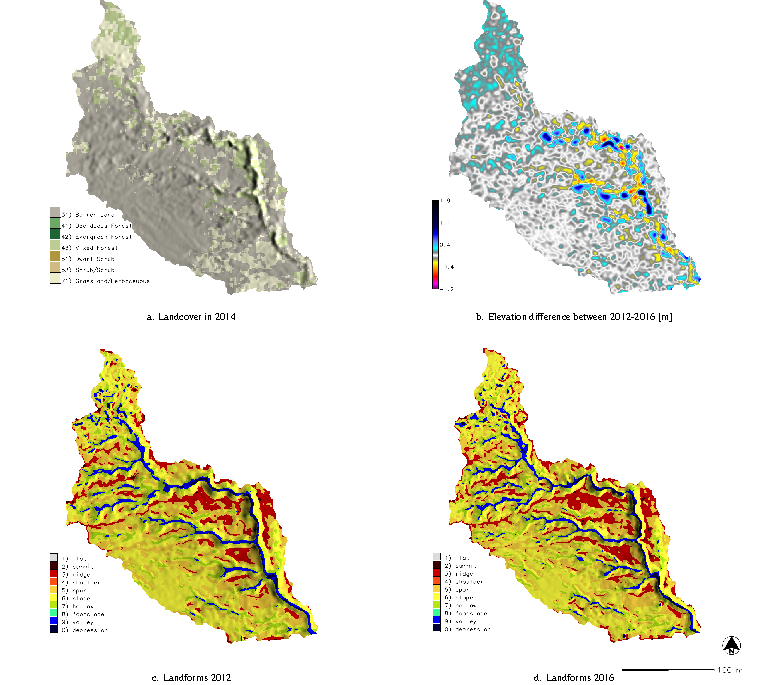
\includegraphics[width=\textwidth,height=0.95\textheight,keepaspectratio]{figures/study_area.pdf}
\caption{Subwatershed, Patterson Branch Creek, Fort Bragg, NC, USA}
\label{fig:study_area}
\end{figure}

% --------- SIMULATIONS ---------
\subsection{Simulations}
%
We ran a sequence of r.sim.terrain simulations 
for the Patterson Branch Creek subwatershed study area
to test dynamic and steady state flow regimes
in the SIMWE, RUSLE3D, and USPED models
(Table~\ref{table:simulations}).
%
RUSLE3D was used to simulate 120~\unit{min} events
with rainfall intensities of 50~\unit{mm~hr}$^{-1}$
for detachment capacity limited soil erosion regimes
for both dynamic and steady state flow regimes
using RUSLE3D
(Figure~\ref{fig:simulations}a-c).
% 
USPED was used to simulate 120~\unit{min} events
with rainfall intensities of \unit{50~mm~hr}$^{-1}$
for transport capacity limited soil erosion regimes
for both dynamic and steady state flow regimes
(Figure~\ref{fig:simulations}d-f).
%
SIMWE was used to simulate 120~\unit{min} events 
with rainfall intensities of 50~\unit{mm~hr}$^{-1}$
for erosion-deposition 
and detachment limited soil erosion regimes 
in steady state flow regimes
(Figure~\ref{fig:simwe_simulations}).
%
In all of the simulations 
a sink filling algorithm
-- an optional parameter in r.sim.terrain -- 
was used to reduce the effects of positive feedback loops
that cause the over-development of scour pits. 

% scripts
The simulations were automated and run in parallel
using Python scripts that are available in the 
\href{https://github.com/baharmon/landscape_evolution}{software repository}.
% reproducibility
The simulations can be reproduced using these scripts
and the study area dataset 
by following the instructions 
in the Open Science Framework repository 
at \url{https://osf.io/tf6yb/}.
% benchmarks
The simulations were run 
in GRASS GIS 7.4 
on a desktop computer 
with 64-bit Ubuntu 16.04.4 LTS,
8 x 4.20 GHz Intel Core i7 7700K CPUs,
and 32 GB RAM. 
% multithreading
Simulations using SIMWE 
are far more computationally intensive
than RULSE3D or USPED, 
but support multi-threading 
when compiled with OpenMP. 
% runtime
Dynamic simulations of RUSLE3D and USPED each took
3~\unit{min}~14~\unit{s} to run on a single thread, 
while steady state simulations for SIMWE each took 
84~\unit{min}~13~\unit{s} running on 6 threads
(Table~\ref{table:simulations}).


% --------- RESULTS ---------
\subsection{Results}

% dynamic model results
The dynamic RUSLE3D simulation
deepened the main channel of the gully,
while the dynamic USPED simulation
eroded the banks of the gully
and deposited in channels
causing the gully grow wider and shallower
(Figure~\ref{fig:simulations}). 
%
As a detachment capacity limited model
RUSLE3D's results were
dominated by erosion and 
thus negative elevation change.
%
RUSLE3D carved a deep incision 
in the main gully channel
where water and sediment flow accumulated
(Figure~\ref{fig:simulations}c). 
%
As a transport capacity limited model
USPED generated a distributed pattern
with both erosion and deposition and thus
negative and positive elevation change. 
%
While USPED's pattern of elevation change
was grainy and fragmented, 
it captured the process of channel 
filling and widening expected with 
a transport capacity limited soil erosion regime
(Figure~\ref{fig:simulations}f). 

% steady state model results
The steady state SIMWE simulations 
predicted more realistic patterns 
of landscape evolution
(Figure~\ref{fig:simwe_simulations}). 
%
For transport limited and
variable erosion-deposition regimes
SIMWE simulated
channel widening 
and the formation of depositional ridges
along the thalweg of the channel
(Figure~\ref{fig:simwe_simulations}c).
%
For a detachment limited soil erosion regime
SIMWE simulated major erosion
driving the continued development 
of the gully network
including the spread of rills and
the evolution of the nascent branch
into a full fledged channel
(Figure~\ref{fig:simwe_simulations}f). 
%
The detachment limited simulation
also formed extensive ridges
beside the gully channels 
(Figure~\ref{fig:simwe_simulations}f), 
continuing the development of 
channel-side ridges
observed in the 2012 and 2016 landform maps
(Figure~\ref{fig:study_area}e-f). 

% comparison of dynamic and steady state results
Given the presence of an active gully 
with ridges along its banks,
this landscape is dominated by 
a detachment limited soil erosion regime.
%
The detachment limited SIMWE simulation 
generated the morphological features
-- the deeply incised gully channels, 
scour pits,
and ridges along the channels 
--
characteristic of its erosion regime,
realistically simulating landscape evolution 
at the scale of a subwatershed. 
%
The erosion-deposition and transport limited 
SIMWE simulations also generated 
the morphological processes and features
that would be expected in these regimes
-- gradual aggradation
and the formation of a depositional ridge 
along the thalweg of the channel.

While RUSLE3D and USPED
produced less realistic patterns of landscape evolution
than SIMWE,
these models were much faster and still generated
the key morphological patterns and processes -- 
channel incision, filling, and widening. 
%
Given their speed
and approximate modeling of erosive processes, 
RUSLE3D and USPED 
are effective for simulating landscape evolution
at regional scales, 
i.e.~for landscapes greater than 10~\unit{km}$^{2}$. 
%
RUSLE3D for example has been used to
model erosion for the entire 650~\unit{km}$^{2}$ 
Fort Bragg installation at 9~\unit{m} resolution
\citep{Levine2018}. 

% --------- SIMULATION TABLE ---------

% table of simulations
\begin{table*}
\small
\caption{Landscape evolution simulations}
\begin{tabu} to \textwidth {XXXXXllllllX}
\toprule
Dynamics & Model & Intensity & Duration & Interval & $D_c$ & $T_c$ & m & n & $\rho_s$ & Threads & Runtime\\
\midrule
Dynamic & RUSLE3D & 50~\unit{mm~hr}$^{-1}$ & 120~\unit{min} & 3~\unit{min} &  &  & 0.4 & 1.3 & & & 2~\unit{min}~36~\unit{s}\\
Dynamic & USPED & 50~\unit{mm~hr}$^{-1}$ & 120~\unit{min} & 3~\unit{min} &  &  & 1.5 & 1.2 & 1.6 & & 3~\unit{min}~14~\unit{s}\\
Steady state & SIMWE & 50~\unit{mm~hr}$^{-1}$ & 120~\unit{min} & 120~\unit{min} & 0.001 & & & & 1.6 & 6 & 84~\unit{min}~13~\unit{s}\\
Steady state & SIMWE & 25~\unit{mm~hr}$^{-1}$ & 120~\unit{min} & 120~\unit{min} & 0.0001 & 0.01 & & & 1.6 & 6 & 84~\unit{min}~13~\unit{s}\\
\bottomrule
\\
\end{tabu}
\label{table:simulations} 
\end{table*}

% --------- SIMULATION FIGURES ---------

% dynamic figure
\begin{figure}
\center
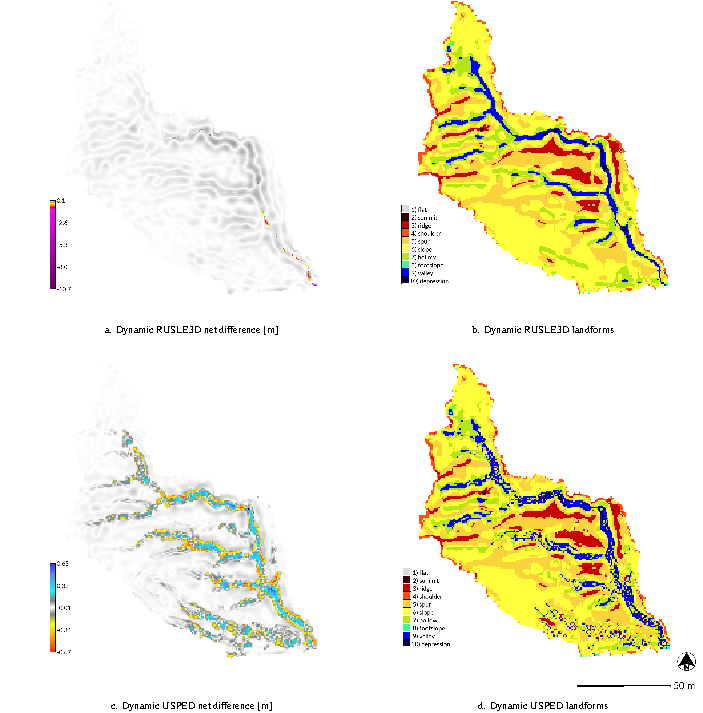
\includegraphics[width=\textwidth,height=0.925\textheight,keepaspectratio]{figures/simulations.pdf}
\caption{Dynamic RUSLE3D and USPED simulations
for a 120~\unit{min} event with a rainfall intensity of 50~\unit{mm~hr}$^{-1}$}
\label{fig:simulations}
\end{figure}

% steady state simwe figure
\begin{figure}
\center
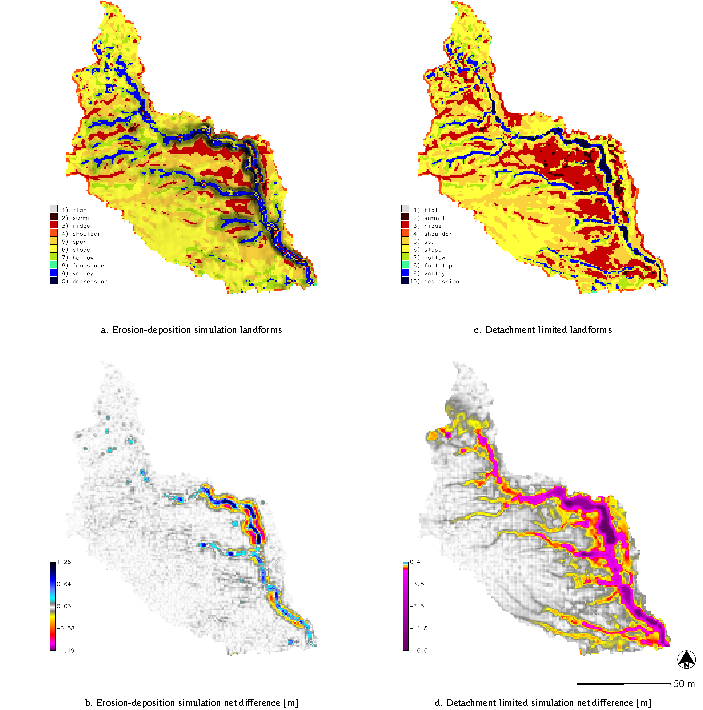
\includegraphics[width=\textwidth,height=0.95\textheight,keepaspectratio]{figures/simwe.pdf}
\caption{Steady state SIMWE simulations
for 120~\unit{min} events with rainfall intensities of 50~\unit{mm~hr}$^{-1}$
and 25~\unit{mm~hr}$^{-1}$}
\label{fig:simwe_simulations}
\end{figure}

% -------------------- CONCLUSIONS ---------------------------------
\conclusions

The short-term landscape evolution model 
r.sim.terrain 
can realistically simulate the development of 
gullies, rills, and hillslopes by overland water erosion
for a range of hydrologic and soil erosion regimes.
The landscape evolution model was tested
with a series of simulations for different 
hydrologic and soil erosion regimes
for a highly eroded sub-watershed on Fort Bragg
with an active gully.
For each regime it generated the 
morphological processes and features expected.
% physics based models
The physics-based SIMWE model 
realistically simulated short-term topographic change
for steady state hydrologic regimes
at sub-watershed to watershed scales. 
For detachment limited soil erosion regimes
it simulated morphological processes including
channel incision, channel widening, and 
the development of knickzones, rills, and scour pits.
For transport limited and variable erosion-deposition regimes,
it simulated processes such as channel aggradation,
scouring, and the development of
depositional ridges along the thalweg.
% empirical models
The empirical RUSLE3D and USPED models
approximated short-term topographic change
at watershed to regional scales. 
For detachment limited soil erosion regimes 
RUSLE3D simulated channel incision,
while for transport limited regimes
USPED simulated channel widening and filling. 
% uses & implications
Since it is a GIS-based model 
that realistically simulates 
fine-scale morphological processes and features,
r.sim.terrain can easily and effectively be used 
in conjunction with other GIS-based tools
for geomorphological research,
land management and conservation,
erosion control, and landscape restoration. 

% --------------------CODE AND DATA------------------------

\codedataavailability{
% open science
As a work of open science
this study is reproducible, repeatable, and recomputable.
Since the data, model, GIS, dependencies are all 
free and open source, the study can easily be reproduced.
% code
The landscape evolution model 
has been implemented in Python as module
for GRASS GIS, a free and open source GIS.
 The source code for the model is hosted on GitHub at 
\url{https://github.com/baharmon/landscape_evolution}
under the GNU General Public License version 2.
The code repository also includes Python scripts 
for running and reproducing the simulations in this paper. 
The digital object identifier (DOI) 
for the version of the software documented in this paper is:
\url{https://doi.org/10.5281/zenodo.2542921}.
% data
The geospatial dataset for the study area is available on GitHub at
\url{https://github.com/baharmon/landscape_evolution_dataset}
under the 
\href{https://opendatacommons.org/licenses/odbl/}{Open Database License} 
with the DOI:
\url{https://doi.org/10.5281/zenodo.2542929}.
% osf
The source code, scripts, data, and results are also hosted
on the Open Science Framework at 
\url{https://osf.io/tf6yb/}
with the DOI:
\url{https://doi.org/10.17605/osf.io/tf6yb}.
} 

% ----------------------------------------------------------------------------

\noappendix 

\authorcontribution{
Brendan Harmon developed 
the models, code, data, case studies, and manuscript.
Helena Mitasova contributed to the development 
of the models and case studies and revised the manuscript.
Anna Petrasova and Vaclav Petras
contributed to the development of the code.
All authors read and approved the final manuscript.
}

\competinginterests{The authors declare that they have no conflict of interest.} 

\begin{acknowledgements}
We acknowledge the GRASS GIS Development Community
for developing and maintaining GRASS GIS.
\end{acknowledgements}

% ---------------------REFERENCES---------------------------
\bibliographystyle{copernicus}
\bibliography{landscape_evolution.bib}

\end{document}
